\documentclass[UTF8]{ctexart} %使用ctex包,中文支持
\usepackage{amsmath}  %数学公式
\usepackage{graphicx} %插图
\usepackage{fancyhdr} %个性化页眉页脚
\usepackage{geometry} %页边距
\usepackage{bm}  % 公式加粗
\usepackage{float} %为了在分栏下插入图片
\usepackage{ulem}  % 换行下划线
%\usepackage{setspace} %行间距
\usepackage{multicol} %用于实现在同一页中实现不同的分栏
\geometry{a4paper,left=2cm,right=2cm,top=2cm,bottom=2cm} % 页边距设置

\title{机器学习笔记}
\author{宋佳欢}
\pagestyle{plain}

\begin{document}
	\maketitle
	\tableofcontents
	\songti \zihao{-4}
	
	\section{支持向量机}
		\begin{multicols}{2}
			\subsection{基本描述}
				SVM算法目的是找到一个最优的超平面,划分给定的数据集D
				\[D=\{(\bm{x_1},y_1),(bm{x_2},y_2),\cdots,(\bm{x_m},y_m)\}\]
				\[y_i\in \{-1,1\}\nonumber\]
				其中划分的超平面可以用如下方程来表达:
				\[\bm{w}^T\bm{x}+b=0\]
				
				例如二维情形时,超平面退化为一条直线,$\bm{w}=[w_1,w_1]^T,\bm{x}=[x_1,x_2]^T$,向量$\bm{w}$的方向与分割超平面垂直,即$\bm{w}$为超平面的法向量,$b$则决定超平面的截距。
				\begin{figure}[H]
					\centering{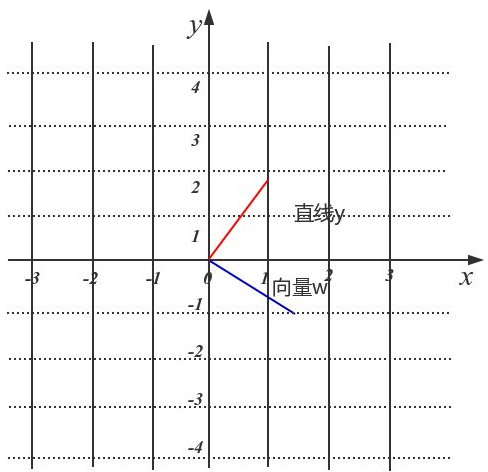
\includegraphics[scale=0.35]{1.png}}
					\caption{\textbf{w}与超平面的关系}
				\end{figure}
				那么什么样的超平面才叫好呢?对于二维情况,我们希望下图2中的虚线上的边界点到超平面的距离越大越好,这样的话对于新的样本分类,才有最大的鲁棒性。由图中可知,超平面的位置仅仅取决于边界上的样本,这些样本被称为支持向量。根据点到直线的距离公式:
				\[d=\bigg|\frac{Ax_0+By_0+C}{\sqrt{A^2+B^2}}\bigg|\]
				其中直线方程为$Ax_0+Bx_0+C=0$,点的坐标为$(x_0,y_0)$,推广到多维情形可得点到超平面的距离公式:
				\[d=\frac{|\bm{w}^T\bm{x}+b|}{\|\bm{w}\|}\]	
				\begin{figure}[H]
					\centering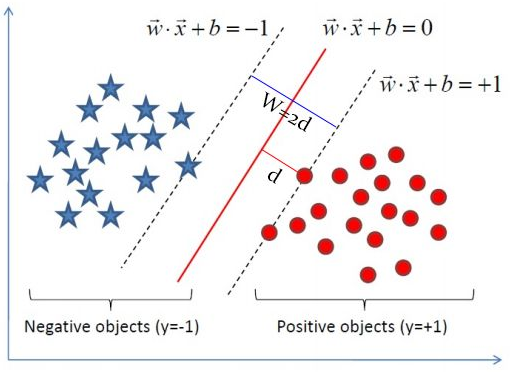
\includegraphics[scale=0.4]{2.png}
					\caption{二维情况的最大间隔分类}
				\end{figure}
				我们希望获得一个超平面,使得其能在正确分类样本的情况下,分类间隔$W$最大。
				
			\subsection{约束条件}
				便于直观理解,从对数几率回归出发,对数几率回归的损失函数为:
				\[L=-(ylogp_{pred}+(1-y)log(1-p_{pred}))\]
				将sigmoid函数与线性部分拆开:
				\[L=-ylog\frac{1}{1+e^{-\bm{\theta}^T\bm{x}}}-(1-y)log(1-\frac{1}{1+e^{-\bm{\theta}^T\bm{x}}})\]
				
				我们将图3中的sigmoid激活函数替换为一个紫红色的分段函数,令$\theta=(\bm{w};b)$当$y=1$,我们希望$\bm{\theta}^T\bm{x}\gg0$,当$y=0$,我们希望$\bm{\theta}^T\bm{x}\ll0$,使得损失函数最小。
				\begin{figure}[H]
					\centering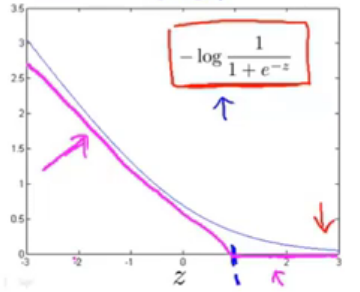
\includegraphics[scale=0.5]{3.png}
					\caption{激活函数替换}
				\end{figure}
				
				\begin{figure}[H]
					\centering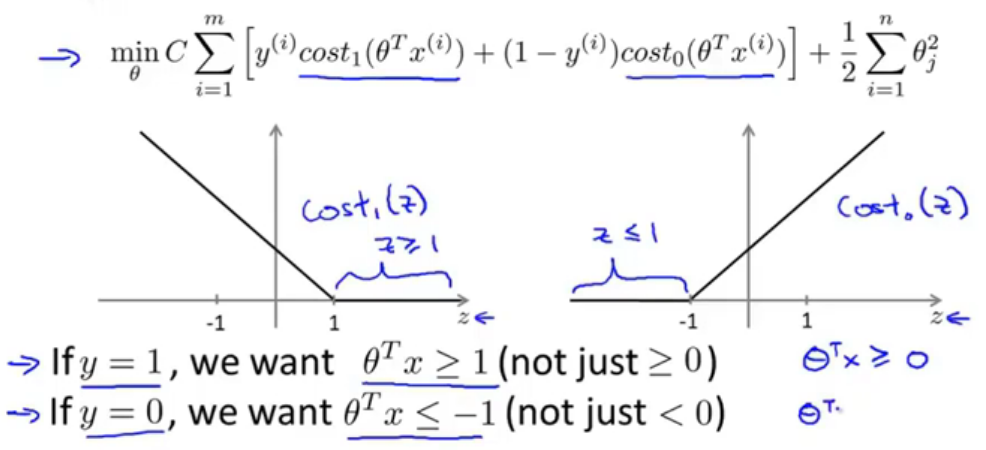
\includegraphics[scale=0.23]{4.png}
					\caption{替换之后的对数几率回归}
				\end{figure}
				
				图4的损失函数中加入了正则化项,超参数C来权衡两者的重要性。对于线性可分的样本,因为有多个超平面满足下式:
				\[\begin{cases}
				\bm{\theta}^T\bm{x}\geq1,y=1\\
				\bm{\theta}^T\bm{x}\leq-1,y=0
				\end{cases}\]
				如下图所示,明显可以看出黑色的要比红色和绿色的好。但是如果没有正则化项,这三个分类器的损失函数都等于0,算法可能会得到其中任何一个。
				\begin{figure}[H]
					\centering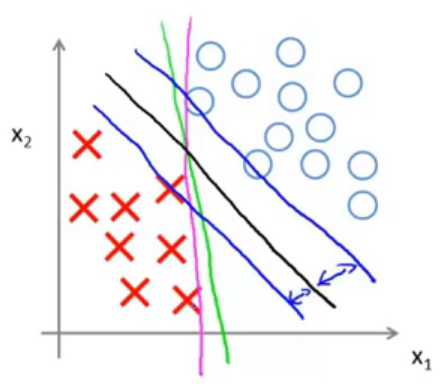
\includegraphics[scale=0.3]{5.png}
					\caption{分开样本的不同超平面}
				\end{figure}
				
				当C取到很大的值时,损失函数的第一项将为0。将标签换成1和-1,方便表述,因此优化问题就可以表示为:
				\begin{align}
				&\quad min\frac{1}{2}\|\bm{w}\|^2\nonumber\\
				s.t.& \quad y_i(\bm{w}^Tx_i+b)\geq1, i=1,2,\dots,n\nonumber
				\end{align}
				
				最小化$w$的直观理解:根据向量内积公式$\bm{w}^T\bm{x}=\|\bm{w}\|\cdot \|\bm{x}\|\cdot cos\alpha$,其中$\alpha$是向量之间的夹角。内积可看成样本$\bm{x}$在$\bm{w}$上的投影乘上$w$的模长。因此我们期望正样本与$w$之间的夹角趋于0,负样本与$w$之间的夹角趋于180。所以$w$的模长最小时,投影的长度会达到最大,达到了我们对夹角的期望。
			\subsection{优化求解}
				最优化问题可分为无约束、等式约束、不等式约束。
				
				无约束优化问题:可以令函数$f(x)$的导数为零来求得。
				
				等式约束优化问题:常常使用的方法就是拉格朗日乘子法(Lagrange Multiplier) ,即把等式约束$h_i(x)$用一个系数与$f(x)$写为一个式子,称为拉格朗日函数,而系数称为拉格朗日乘子。通过拉格朗日函数对各个变量求导,令其为零,可以求得候选值集合,然后验证求得最优值。
				
				不等式约束优化问题:常常使用的方法就是KKT条件。同样地,我们把所有的等式、不等式约束与f(x)写为一个式子,也叫拉格朗日函数,系数也称拉格朗日乘子,通过一些条件,可以求出最优值的必要条件,这个条件称为KKT条件。
				
				\subsubsection{拉格朗日函数}
					首先,我们先要从宏观的视野上了解一下拉格朗日对偶问题出现的原因和背景。
					
					我们知道我们要求解的是最小化问题,所以一个直观的想法是如果我能够构造一个函数,使得该函数在可行解区域内与原目标函数完全一致,而在可行解区域外的数值非常大,甚至是无穷大,那么这个没有约束条件的新目标函数的优化问题就与原来有约束条件的原始目标函数的优化问题是等价的问题。这就是使用拉格朗日方程的目的,它将约束条件放到目标函数中,\uline{从而将有约束优化问题转换为无约束优化问题。}
					
					随后,人们又发现,使用拉格朗日获得的函数,使用求导的方法求解依然困难。进而,需要对问题再进行一次转换,即使用一个数学技巧:\uline{拉格朗日对偶。}
					
					因此在拉格朗日优化问题上,需要进行两个步骤:
					
					(1)将有约束的原始目标函数转换为无约束的新构造的拉格朗日目标函数。
					
					(2)使用拉格朗日对偶性,将不易求解的优化问题转化为易求解的优化。
					
					\uline{第一步:将有约束的原始目标函数转换为无约束的新构造的拉格朗日目标函数。}
					\[L(\bm{w},b,\bm{\alpha}) = \frac{1}{2}\|\bm{w}\|^2 - 
					\sum_{i=1}^n \alpha_i\big(y_i(\bm{w}^T\bm{x}_i+b)-1\big)\]
					
					其中$\alpha_i$是拉格朗日乘子,且$\alpha\geq0$。令:
					\[\theta (\bm{w}) = \max_{\alpha_i\geq0}L(\bm{w},b,\bm{\alpha})\]
				
					当样本点不满足约束条件时,即在可行解区域外:
					\[y_i(\bm{w}^Tx_i+b)<1\]
					此时,我们将$\alpha_i$设置为正无穷,此时$\theta(\bm{w})$显然也是正无穷。
				
					当样本点满足约束条件时,即在可行解区域内:
					\[y_i(\bm{w}^Tx_i+b)\geq1\]
					
					将以上两种情况结合,得到新的目标函数:
					\[\begin{cases}
						\frac{1}{2}\|\bm{w}\|^2\quad x\in feasible\; domain\\
						+\infty \quad x\in non-feasible\; domain
					\end{cases}\]
					
					再看我们的初衷,就是为了建立一个在可行解区域内与原目标函数相同,在可行解区域外函数值趋近于无穷大的新函数,现在我们做到了。 我们的问题变成了求新目标函数的最小值,即:
					\[\min_{\bm{w},b}\theta(\bm{w}) = \min_{\bm{w},b}\max_{\alpha_i\geq0}L(\bm{w},b,\bm{\alpha})=p^*\]
					这里用p*表示这个问题的最优值,且和最初的问题是等价的。
					
					\uline{第二步:将不易求解的优化问题转化为易求解的优化。}
					我们看一下我们的新目标函数,先求最大值,再求最小值。这样的话,我们首先就要面对带有需要求解的参数$\bm{w}$和$b$的方程,而$\alpha_i$又是不等式约束,这个求解过程不好做。所以,我们需要使用拉格朗日函数对偶性,将最小和最大的位置交换一下,这样就变成了:
					\[\max_{\alpha_i\geq0}\min_{\bm{w},b}L(\bm{w},b,\bm{\alpha})=d^*\]
					交换以后的新问题是原始问题的对偶问题,这个新问题的最优值用d*来表示。而且d*<=p*。因为p是先求最大的一块区域然后在这块区域求最小,d是先求最小的一块区域然后在这块区域求最大,最大里面的最小,总会比最小里面的最大要大(或等于)。
								
					d*<=p*,称为弱对偶,对于所有优化问题都成立,这个时候我们可以得到原始问题的一个下界。
					
					如果d*=p*,称为强对偶,满足某些条件才成立,这时可以用解对偶问题替代原始问题。那么满足什么样的条件可以得到强对偶呢?
					
					如果原问题是一个凸优化,并且不等式约束是严格可行的。					
					,那么强对偶成立。这里需要注意的是,这里的条件只是强对偶成立的一种情况,对于非凸的问题也有可能是强对偶。
					
					强对偶成立时,将拉格朗日函数分别对原变量x和对偶变量$\alpha$和$\beta$分别求导,令导数等于零(还需要满足KKT条件),即可求解对偶问题的解,也就求得了原问题的解。
					
					
					
		\end{multicols}
		
	
	
		
\end{document}